% Trying to break the document up a bit.  This command simply inserts the contents of the file at this point.  It contains the document license, preamble, and title page: things that aren't likely to change more than once.  This can be used to separate discrete parts of a document into files that are easier to edit at one time.
%%%%%%%%%%%%%%%%%%%%%%%%%%%%%%%%%%%%%%%%%%%%%%%%%%%%%%%%%%%%%%%%%%%%%%
% This layout was adapted from one found at latextemplates.com which
% was adapted from another.
%
% License: CC BY-NC-SA 3.0
% (http://creativecommons.org/licenses/by-nc-sa/3.0/)
%
% Original header:
%
% This is a LaTeX version of the sample laboratory report from
% Virginia Tech's copyrighted 08-09 CHEM 1045/1046 lab manual.
% Reproduction of this one appendix section for academic purposes
% should fall under fair use.
%
%%%%%%%%%%%%%%%%%%%%%%%%%%%%%%%%%%%%%%%%%%%%%%%%%%%%%%%%%%%%%%%%%%%%%%

\documentclass{article}

\usepackage{graphicx}
% \usepackage[acronym]{glossaries} % Lets us use acronyms
\usepackage{multicol}
\usepackage{amsmath}
\usepackage{siunitx} % SI units in math mode
\usepackage{subcaption}

\author{}
\title{ELEC-313 \\ Lab 5: CMOS Circuits\\ }
\date{\today}

% \loadglsentries{acronyms} % Actually loads 'acronyms.tex'
% \makeglossaries

\begin{document}

\maketitle

\begin{center}
  \begin{tabular}{lr}
    Date Performed: & October 16, 2013 \\
    Partners:       & Charles Pittman    \\
    & Stephen Wilson     \\
  \end{tabular}
\end{center}

\newpage

\tableofcontents
\listoffigures
\listoftables
\newpage

% Number the enumerate environment (unordered lists) by letter:
\renewcommand{\labelenumi}{\alph{enumi}.}

\section{Objective}
\label{sec:objective}

The objective is to construct and observe the operation of a CMOS inverter and NAND gate.

\section{Equipment}
\label{sec:equipment}

\begin{itemize}
\item ALD1105 Dual N-channel and P-channel matched pair MOSFET
\item Power supply: HP E3631A
\item Oscilloscope: Agilent 54622D
\item Function generator: HP 33120A
\end{itemize}

 \section{Schematics}
 \label{sec:schematics}

 % \begin{figure}[hbtp]
 %   \centering
 %   \begin{subfigure}[b]{0.4\textwidth}
 %     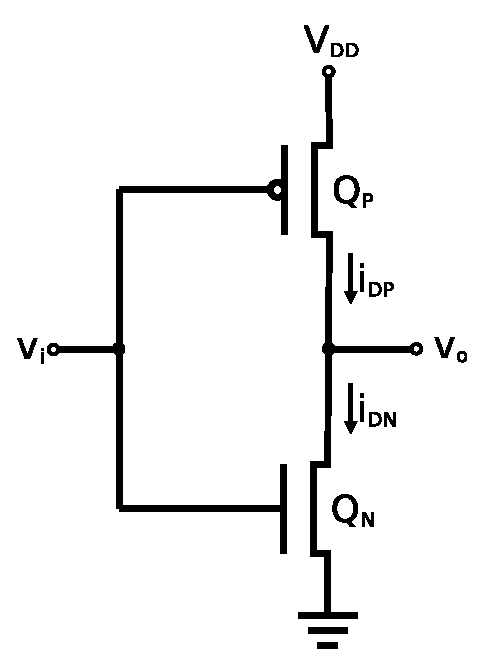
\includegraphics[width=\textwidth]{invert}
 %     \caption{\label{schem:inverter} CMOS Inverter}
 %   \end{subfigure}%
 %   ~
 %   \begin{subfigure}[b]{0.4\textwidth}
 %     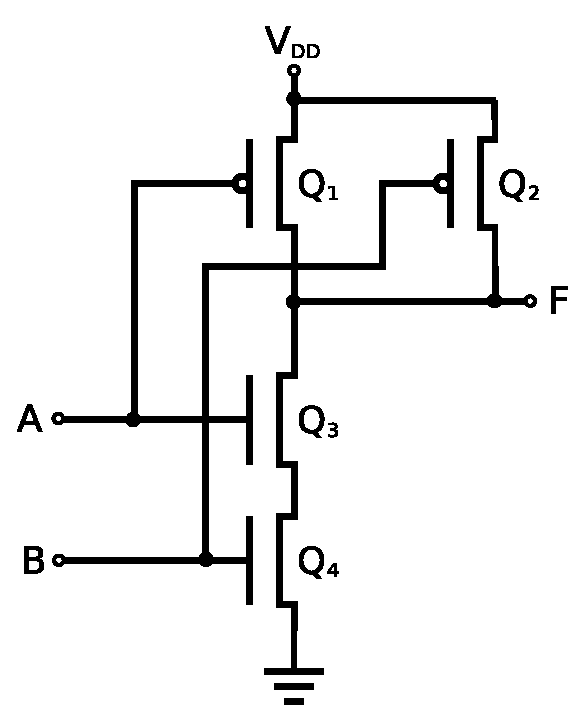
\includegraphics[width=\textwidth]{nand}
 %     \caption{\label{schem:nand} CMOS NAND}
 %   \end{subfigure}
 %   \caption{\label{fig:schematics} Circuits used in this lab.}
 % \end{figure}

\section{Procedure}
\label{sec:procedure}

\subsection{CMOS Inverter}
\label{sec:inverter}

\begin{enumerate}
\item Construct the circuit of Figure~\ref{schem:inverter}.
\item Connect the \si{V+} terminal (Pin 11) to the + supply voltage
\item Connect the \si{V-} terminal (Pin 4) to the circuit ground.
\item Set VDD to \SI{5}{V} using the HP source.
\item Use the function generator to input $V_i$. Set the function generator to a frequency of \SI{20}{kHz} and select a triangle wave. Set the wave for 0 to \SI{5}{V} using the offset.
\item Connect channel 1 of the oscilloscope to the input and channel 2 to the output.
\item Use the x-y plot function of the scope to produce the transfer characteristic $V_o$ vs. $V_i$. (Press the main key, then select the x-y soft-key, then adjust the voltage scales as needed.)
\item Capture the $V_o$ vs. $V_i$.  data, so you can recreate the plot for the lab report.
\item Adjust the amplitude and offset of the function generator for an input square wave of 0 to \SI{5}{V} as measured on the oscilloscope.
\item Adjust the scope and capture both input and output on one screen for the report.
\item Measure the propagation delay times of the output waveform.
\end{enumerate}

\subsection{CMOS NAND}
\label{sec:nand}

\begin{enumerate}
\item Construct the circuit of figure~\ref{schem:nand}.
\item Connect the \si{v+} terminal (Pin 11) to the + supply voltage.
\item Connect the \si{V-} terminal (Pin 4) to the circuit ground.
\item Set the + supply voltage to \SI{5}{V} DC using the HP source.
\item Set input A to \SI{0}{V}.
\item Use the function generator for input B. Set the function generator to a frequency of \SI{20}{kHz} and select a square wave. Set the square wave for 0 to \SI{5}{V} using the offset.
\item Connect channel 1 of the oscilloscope to the input and channel 2 to the output.
\item Adjust the scope and capture both input and output on one screen for the report.
\item Repeat step 8 with the input A set to +\SI{5}{V}.
\end{enumerate}

\newpage

\section{Results}
\label{sec:results}

\begin{figure}[hbtp]
  \centering
  \resizebox{1.0\textwidth}{!}{% GNUPLOT: LaTeX picture with Postscript
\begingroup
  \makeatletter
  \providecommand\color[2][]{%
    \GenericError{(gnuplot) \space\space\space\@spaces}{%
      Package color not loaded in conjunction with
      terminal option `colourtext'%
    }{See the gnuplot documentation for explanation.%
    }{Either use 'blacktext' in gnuplot or load the package
      color.sty in LaTeX.}%
    \renewcommand\color[2][]{}%
  }%
  \providecommand\includegraphics[2][]{%
    \GenericError{(gnuplot) \space\space\space\@spaces}{%
      Package graphicx or graphics not loaded%
    }{See the gnuplot documentation for explanation.%
    }{The gnuplot epslatex terminal needs graphicx.sty or graphics.sty.}%
    \renewcommand\includegraphics[2][]{}%
  }%
  \providecommand\rotatebox[2]{#2}%
  \@ifundefined{ifGPcolor}{%
    \newif\ifGPcolor
    \GPcolortrue
  }{}%
  \@ifundefined{ifGPblacktext}{%
    \newif\ifGPblacktext
    \GPblacktextfalse
  }{}%
  % define a \g@addto@macro without @ in the name:
  \let\gplgaddtomacro\g@addto@macro
  % define empty templates for all commands taking text:
  \gdef\gplbacktext{}%
  \gdef\gplfronttext{}%
  \makeatother
  \ifGPblacktext
    % no textcolor at all
    \def\colorrgb#1{}%
    \def\colorgray#1{}%
  \else
    % gray or color?
    \ifGPcolor
      \def\colorrgb#1{\color[rgb]{#1}}%
      \def\colorgray#1{\color[gray]{#1}}%
      \expandafter\def\csname LTw\endcsname{\color{white}}%
      \expandafter\def\csname LTb\endcsname{\color{black}}%
      \expandafter\def\csname LTa\endcsname{\color{black}}%
      \expandafter\def\csname LT0\endcsname{\color[rgb]{1,0,0}}%
      \expandafter\def\csname LT1\endcsname{\color[rgb]{0,1,0}}%
      \expandafter\def\csname LT2\endcsname{\color[rgb]{0,0,1}}%
      \expandafter\def\csname LT3\endcsname{\color[rgb]{1,0,1}}%
      \expandafter\def\csname LT4\endcsname{\color[rgb]{0,1,1}}%
      \expandafter\def\csname LT5\endcsname{\color[rgb]{1,1,0}}%
      \expandafter\def\csname LT6\endcsname{\color[rgb]{0,0,0}}%
      \expandafter\def\csname LT7\endcsname{\color[rgb]{1,0.3,0}}%
      \expandafter\def\csname LT8\endcsname{\color[rgb]{0.5,0.5,0.5}}%
    \else
      % gray
      \def\colorrgb#1{\color{black}}%
      \def\colorgray#1{\color[gray]{#1}}%
      \expandafter\def\csname LTw\endcsname{\color{white}}%
      \expandafter\def\csname LTb\endcsname{\color{black}}%
      \expandafter\def\csname LTa\endcsname{\color{black}}%
      \expandafter\def\csname LT0\endcsname{\color{black}}%
      \expandafter\def\csname LT1\endcsname{\color{black}}%
      \expandafter\def\csname LT2\endcsname{\color{black}}%
      \expandafter\def\csname LT3\endcsname{\color{black}}%
      \expandafter\def\csname LT4\endcsname{\color{black}}%
      \expandafter\def\csname LT5\endcsname{\color{black}}%
      \expandafter\def\csname LT6\endcsname{\color{black}}%
      \expandafter\def\csname LT7\endcsname{\color{black}}%
      \expandafter\def\csname LT8\endcsname{\color{black}}%
    \fi
  \fi
  \setlength{\unitlength}{0.0500bp}%
  \begin{picture}(7200.00,5040.00)%
    \gplgaddtomacro\gplbacktext{%
      \csname LTb\endcsname%
      \put(726,440){\makebox(0,0)[r]{\strut{}0mA}}%
      \csname LTb\endcsname%
      \put(726,1307){\makebox(0,0)[r]{\strut{}5mA}}%
      \csname LTb\endcsname%
      \put(726,2174){\makebox(0,0)[r]{\strut{}10mA}}%
      \csname LTb\endcsname%
      \put(726,3041){\makebox(0,0)[r]{\strut{}15mA}}%
      \csname LTb\endcsname%
      \put(726,3908){\makebox(0,0)[r]{\strut{}20mA}}%
      \csname LTb\endcsname%
      \put(726,4775){\makebox(0,0)[r]{\strut{}25mA}}%
      \csname LTb\endcsname%
      \put(858,220){\makebox(0,0){\strut{}0 V}}%
      \csname LTb\endcsname%
      \put(1453,220){\makebox(0,0){\strut{}2 V}}%
      \csname LTb\endcsname%
      \put(2047,220){\makebox(0,0){\strut{}4 V}}%
      \csname LTb\endcsname%
      \put(2642,220){\makebox(0,0){\strut{}6 V}}%
      \csname LTb\endcsname%
      \put(3236,220){\makebox(0,0){\strut{}8 V}}%
      \csname LTb\endcsname%
      \put(3831,220){\makebox(0,0){\strut{}10 V}}%
      \csname LTb\endcsname%
      \put(4425,220){\makebox(0,0){\strut{}12 V}}%
      \csname LTb\endcsname%
      \put(5020,220){\makebox(0,0){\strut{}14 V}}%
      \csname LTb\endcsname%
      \put(5614,220){\makebox(0,0){\strut{}16 V}}%
      \csname LTb\endcsname%
      \put(6209,220){\makebox(0,0){\strut{}18 V}}%
      \csname LTb\endcsname%
      \put(6803,220){\makebox(0,0){\strut{}20 V}}%
    }%
    \gplgaddtomacro\gplfronttext{%
      \csname LTb\endcsname%
      \put(5816,4602){\makebox(0,0)[r]{\strut{}$I_B = $SI{20}{microampere}}}%
      \csname LTb\endcsname%
      \put(5816,4382){\makebox(0,0)[r]{\strut{}$I_B = $SI{50}{microampere}}}%
      \csname LTb\endcsname%
      \put(5816,4162){\makebox(0,0)[r]{\strut{}$I_B = $SI{80}{microampere}}}%
      \csname LTb\endcsname%
      \put(5816,3942){\makebox(0,0)[r]{\strut{}$I_B = $SI{100}{microampere}}}%
    }%
    \gplbacktext
    \put(0,0){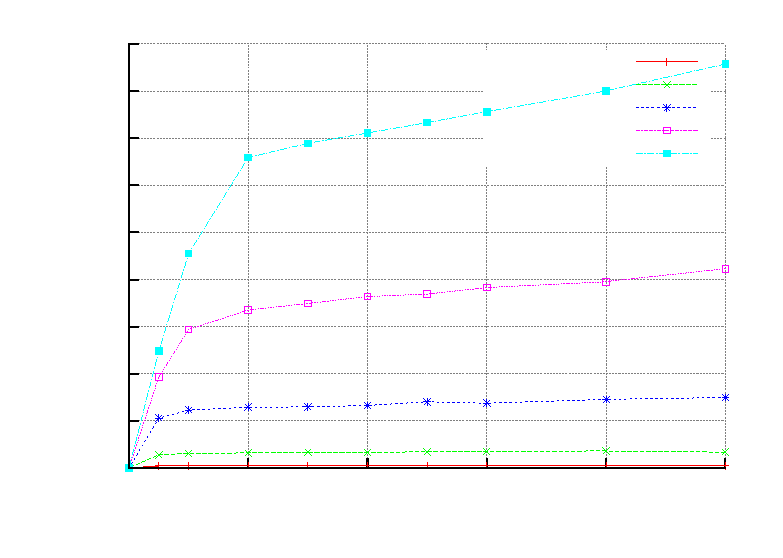
\includegraphics{graph}}%
    \gplfronttext
  \end{picture}%
\endgroup
}
  \caption{\label{fig:graph} Graph}
\end{figure}

\begin{table}[hbtp]
  \centering
  \begin{tabular}{cc|c}
    A & B & F \\
    \hline
    0 & 0 & 1 \\
    0 & 1 & 1 \\
    1 & 0 & 1 \\
    1 & 1 & 0 \\
  \end{tabular}
  \caption{\label{tab:nand} NAND logic table}
\end{table}

\section{Conclusion}
\label{sec:conclusion}

As seen in Figure~\ref{fig:inverter}, as the input voltage ($V_i$) is low (\SI{0}{V}), $V_o$ is high (\SI{5}{V}).  Conversely, when $V_i$ is high, $V_o$ is low. This relationship of $V_i$ to $V_o$ is why the configuration is called an inverter.  Also, the transition from high to low on the output happens when the input is approximately between 1 and \SI{3}{V} at $V_i$; that is, when the input voltage is less than one, the output voltage is almost exactly \SI{5}{V} and when the input voltage is greater than \SI{3}{V}, the output voltage is almost exactly \SI{0}{V}.  (Refer to Figure~\ref{fig:inverter} for a close up of the $V_i$ to $V_o$).  Additionally, the output voltage closely represents a square wave or an on/off relationship as the input voltage is swept back and forth between low and high.  It should also be noted that it takes \SI{58.8}{\nano\second} for the output voltage response to change from high to low.

The circuit in Figure~\ref{schem:nand} operates as a NAND gate (see Table~\ref{tab:nand}) because when input A is low (\SI{0}{V}), the inverting gate ($Q_1$) is shorted and the non-inverting gate ($Q_3$) is open.  Therefore no matter what input B is shown, the output voltage is high.  When input A is high, $Q_1$ is inverted and therefore open and $Q_3$ is shorted. During this state, when input B is low, $Q_2$ is inverted and shorted allowing current to flow through it, but $Q_4$ is open blocking the current and the output voltage is again high.  The only time the output voltage is low, is when A and B are high, which means both the inverting gates $Q_1$ and $Q_2$ are open.  This behavior is shown in Figure~\ref{fig:nand}.

%% Rewrote this part before reading the previous paragraph.  This information has already been given (less the graph and logic table.)
%Figure~\ref{fig:nand} illustrates the NAND gate logic table (Table~\ref{tab:nand}) exactly.  When input A is low, $V_o$ is high whether input B is high or low.  When input A is high, $V_o$ is high while input B is low; when input B goes high, $V_o$ drops to low.

% \section{Equations}
% \label{sec:equations}

% % LaTeX sees blank lines as a start of another paragraph.  To avoid
% % unnecessary vertical spaces between equations, and still visually
% % separate in source, put a comment between them.
% %
% \begin{equation}
%   \label{eq:percent_diff}
%   \%_{diff} = \frac{|nominal - measured|}{nominal}\times 100\%
% \end{equation}
% %
% \begin{equation}
%   \label{eq:ripple}
%   V_r = V_{max} - V_{min}
% \end{equation}
% %
% \begin{equation}
%   \label{eq:volt_reg}
%   \%_{reg} = \frac{V_{load} - V_{no load}}{V_{no load}}\times 100\%
% \end{equation}

\end{document}
